\documentclass[11pt]{article}
\usepackage[a4paper,margin=1.9cm]{geometry}
\usepackage{amsmath,amssymb}
\usepackage{graphicx}
\usepackage{enumitem}
\usepackage[colorlinks=true,urlcolor=blue!50!black]{hyperref}
\usepackage{xcolor}

\graphicspath{{../figures/}}
% Generated by scripts/make_tables.py from results/summary/. Do not edit.
\newcommand{\numdHRKfourLast}{$1.6\times10^{-8}$}
\newcommand{\numdHDOPLast}{$2.5\times10^{-7}$}
\newcommand{\numdHGLtwo}{$5.0\times10^{-12}$}
\newcommand{\numdHGLthreeLast}{$6.7\times10^{-16}$}
\newcommand{\numexpGLthree}{0.48}
\newcommand{\numphaseDOPend}{$1.5\times10^{-3}$}
\newcommand{\numphaseGLthreeEnd}{$7.3\times10^{-11}$}
\newcommand{\numcrossRKfour}{3364}
\newcommand{\numshortDOP}{$776$}
\newcommand{\numshortGLthree}{$5.4\times10^{3}$}
\newcommand{\numlongDOPfour}{$706$}
\newcommand{\numlongGLthreeFour}{$2.1\times10^{3}$}
\newcommand{\numlongGLthreeEight}{$6.2\times10^{3}$}
\newcommand{\numpsDOPdecade}{0.33}
\newcommand{\numpsRKfourDecade}{1.45}
\newcommand{\numpsGLthreeDecade}{2.26}
\newcommand{\numpsGLthreeSaturation}{6.0}
\newcommand{\numpsPlainRKfour}{14.5}
\newcommand{\numpsCompRKfour}{5.0}
\newcommand{\numiscoDPfive}{-0.252}
\newcommand{\numiscoGLtwo}{1.09}
\newcommand{\numiscoGLthree}{1.53}
\newcommand{\numcircPlain}{$5.5\times10^{-6}$}
\newcommand{\numcircComp}{$5.1\times10^{-11}$}
\newcommand{\numcircPlainExp}{2.05}

\pagestyle{empty}
\setlist{nosep,leftmargin=1.2em}
\setlength{\parskip}{0.45em}
\setlength{\parindent}{0pt}

\begin{document}

{\Large\bfseries Geometric versus classical integrators for black-hole geodesics}\\[0.3em]
{\large Research summary} \hfill Nugie Saputra \textperiodcentered{}
\href{https://github.com/NugiePhysics/geodesic-integrators}{github.com/NugiePhysics/geodesic-integrators}

\textbf{Question.} Black-hole imaging traces millions of short photon paths; inspiral
modelling follows a few orbits for thousands of revolutions. Which numerical integrator
should each use, and why? I compared eight integrators on geodesics of the Schwarzschild
metric: classical and adaptive Runge--Kutta (RK4, DP5, DOP853), Gauss--Legendre collocation of
order 2, 4 and 6, and Tao's explicit symplectic scheme. Each runs on the second-order geodesic
equation and on Hamilton's equations, and every error is measured against an exact solution
built from elliptic integrals and functions, for light deflection, the photon sphere, circular
and eccentric orbits, the ISCO and inclined orbits.

\begin{minipage}[t]{0.50\textwidth}
\vspace{0pt}
\textbf{Findings.}
\begin{itemize}
\item \emph{Error growth.} Over $10^4$ orbits the Runge--Kutta methods drift linearly in the
  mass shell (RK4: \numdHRKfourLast) and quadratically in phase; the symplectic methods stay
  bounded (GL2: \numdHGLtwo) with linear phase error. Sixth-order Gauss--Legendre reaches
  round-off and follows Brouwer's $N^{1/2}$ law.
\item \emph{Formulation.} In Hamilton's form, energy and angular momentum are exact for every
  method; the second-order form loses up to 440 times in accuracy near the critical impact
  parameter. A method that is merely symmetric there conserves as well as a symplectic one.
\item \emph{Cost.} DOP853 is cheapest for short integrations at every accuracy. Over 1000
  orbits only sixth-order Gauss--Legendre reaches a phase error of $10^{-8}$
  (\numlongGLthreeEight{} evaluations per orbit).
\item \emph{Edges of stability.} On the photon sphere accuracy buys survival only as
  $\ln 10/2\pi$ orbits per decade, capped near six orbits in double precision; plain
  summation fakes a longer life. At the ISCO the time to plunge scales as
  $|\varepsilon|^{-1/4}$ in the error size, and the error's sign decides whether the orbit
  plunges at all.
\end{itemize}
\end{minipage}\hfill
\begin{minipage}[t]{0.47\textwidth}
\vspace{0pt}
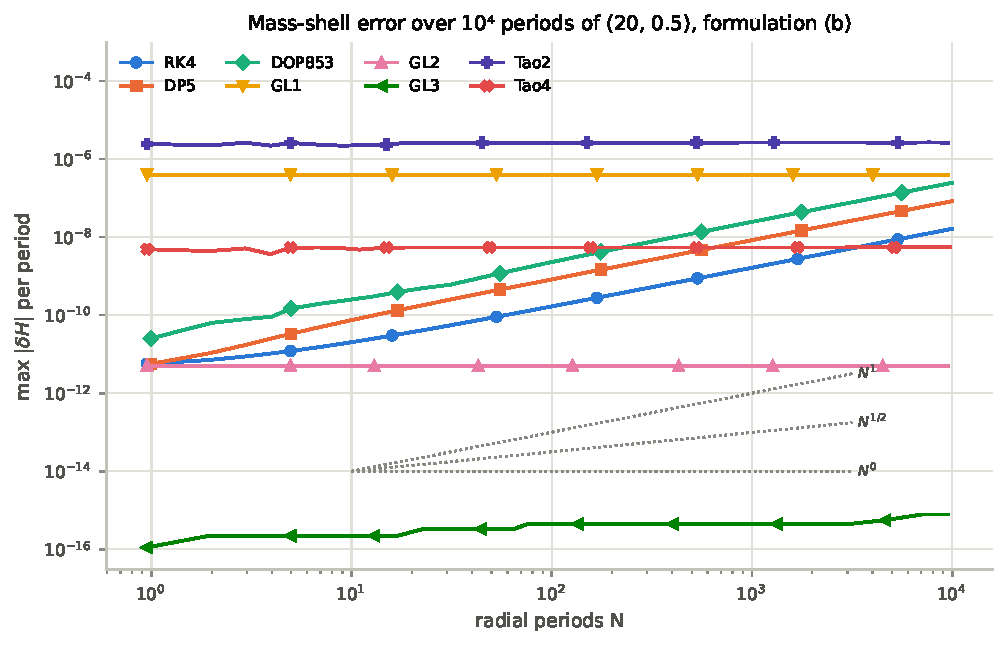
\includegraphics[width=\textwidth]{F07_energy_long_term.pdf}\\[-0.3em]
{\small Mass-shell error over $10^4$ radial periods of an eccentric orbit: linear drift for the
Runge--Kutta methods, bounded error for the symplectic ones, Brouwer's law for GL3 at
round-off.}
\end{minipage}

\textbf{How.} The code (Python with Numba) keeps the full eight-dimensional phase space, so
conserved quantities are measured, not imposed, and separates integrators from physics: they
see only a vector field. Every figure and table is regenerated from a clean checkout by one
command, and a repeated run reproduced every result byte for byte. A development log records
what failed and why, from a mistranscribed elliptic formula caught by an independent check to
an integrator parameter that fails on marginally stable orbits.

\textbf{Next.} The metric interface takes the full inverse metric and its derivatives, so the
Kerr metric enters as a new class with no change to the integrators. This connects directly to
my earlier work on light deflection in Kerr--(anti-)de~Sitter spacetimes: the same framework
can test numerical deflection angles against analytic results where no closed form for the
whole orbit exists, and extend the stability results here to rotating black holes.

\end{document}
